\section{Experiments}
\label{sec:experiments}
\subsection{Protocol, baselines, and inferential units}
\paragraph{Constructed benchmark.}
The resource-participation simulator contains 128 agents, eight time steps, and three trajectory channels. Its mechanism bank has 200 candidates: ten attention values, ten participation values, and two dropout values. Eight seeds represent each candidate. Four historical activities and four accessible-rule probes support calibration and acquisition; development and test each contain three interacting activities. Waiting and forwarding occur separately in history, but conflicts are activated only in probes and later splits. Thus not every rule component has empirical training coverage. The true parameter is $(0.90,0.30,0.27)$, so its dropout coordinate is not exactly represented in the two-level candidate grid. Historical audits contain 96 intent records with 20\% missingness; the acquisition pool contains 160 records with 15\% missingness, generated MCAR. All costs are one record. Candidate paths share simulation random numbers; truth uses separate seeds. The internal name \texttt{SocioVerse\_Campus} denotes this constructed benchmark, not official SocioVerse data.

\paragraph{Frozen selection and evaluation.}
An automated research controller proposed and evaluated 60 distinct modifications of the sole algorithm file. Ten were retained and 50 reverted, with every hypothesis and source version archived. The fixed evaluator, budget grid $\{0,2,4,8,12,16\}$, and cache were not optimized during this loop. The best method was frozen before the first reported test evaluation. Later reruns verify reproduction and are not new holdouts. The original metric is normalized trapezoidal AUC of pooled trajectory RMSE:
\begin{equation}
 A_{\mathrm{pool}}=\frac1{16}\sum_{j=1}^{J}
 (b_j-b_{j-1})\frac{R_{\mathrm{pool}}(b_j)+R_{\mathrm{pool}}(b_{j-1})}{2}.
 \label{eq:auc}
\end{equation}
Trajectory errors use population fractions. The original three events share people, budget and conflicts, so their time points cannot be treated as independent samples.

To quantify variability, a post-freeze supplemental protocol generated 24 independent worlds with population and rollout variation while fixing training observations, acquisition evidence, and three activity templates. For each template we compute $A_e$ by replacing pooled RMSE in Eq.~\eqref{eq:auc} with within-event RMSE, and define $A_{\mathrm{macro}}=\frac13\sum_e A_e$. Whole-world bootstrap resampling (2,000 draws, fixed seed) preserves dependence between activities. Random-query repetitions are averaged inside each world. Tables report each template's 24 independent realizations and conditional 95\% intervals; they do not represent 72 unrelated activities, new training datasets, or new domains. The supplement was specified after the original test had been inspected and is reported as a post-freeze extension, not a prospectively untouched second benchmark.

\paragraph{Comparison policies.}
Random selects available records uniformly. Entropy maximizes binary predictive entropy per cost. ParamIG uses $h(q_r)-\sum_mw_mh(p_{mr})$, where $h$ is binary entropy. Standard OED uses predictive variance reduction directed at historical trajectories rather than combination probes; it represents this specific goal choice, not all goal-oriented design. The original policies begin from uniform compatible weights, while Full begins from Eq.~\eqref{eq:weights}. We therefore add matched-prior versions to isolate acquisition. Passive baselines include a simple historical-mean model, an uncalibrated mixture, process-only and trajectory-only calibration, and passive V1 joint calibration. These are synthetic statistical baselines, not substitutes for unexecuted original-product or LLM baselines.

\subsection{RQ1: Does a compatible set preserve useful mechanism uncertainty?}
The final hard set contains 170 candidates, but only 12 have nonzero float32 weights, and only two exceed $10^{-4}$. The initial effective size $(\sum_mw_m^2)^{-1}$ is \ESS, with largest weight \MaxWeight. The most heavily weighted mechanism is approximately $(0.4167,0.6833,0.42)$, markedly different from the generating attention and participation values. Low trajectory error thus does not establish mechanism recovery.

An additional ambiguity check selects a candidate pair using history and probes, without test outcomes. Its historical pairwise trajectory RMSE is \HistoryPair, and its probe RMSE is \ProbePair. The pair has different parameters, but this observed pair does \emph{not} demonstrate a dramatic amplification of disagreement on combinations. The motivating ambiguity remains a scientifically plausible problem; this diagnostic alone is insufficient to claim that the benchmark realizes its strongest form.

The original single-point baseline uses a different point-selection loss from Full. A matched MAP control instead places all mass on the largest-weight candidate under the evolved calibration. Table~\ref{tab:macro} shows that Full's macro AUC is \MacroFull, compared with \MacroMAP\ for matched MAP. This difference is negligible on the population-fraction scale. Table~\ref{tab:paired} provides paired activity differences rather than inferring significance from overlap of marginal intervals. The results do not establish that preserving the mixture improves accuracy materially.
\begin{table}[tbp]
\centering
\caption{Macro AUC $\times10^3$ and descriptive mean differences. Intervals are world-bootstrap intervals on the mean, not predictive intervals.}
\label{tab:macro}
\scriptsize
\setlength{\tabcolsep}{3pt}
\begin{tabular}{lrr}
\toprule
Method & Macro AUC & Difference from Full \\
\midrule
Full & 7.0635 [6.0247, 8.0995] & +0.0000 \\
Matched MAP & 7.0655 [6.0267, 8.1012] & +0.0019 \\
Matched-prior Random & 7.0589 [6.0192, 8.0962] & -0.0046 \\
Without combination target & 7.0635 [6.0247, 8.0995] & +0.0000 \\
Without batch conditioning & 7.0635 [6.0247, 8.0995] & +0.0000 \\
Without sharing* & 39.8238 [38.5402, 41.0323] & +32.7602 \\
\bottomrule
\end{tabular}
\end{table}


\paragraph{Unknown-rule diagnostics.}
We separately introduce unmodeled waiting dropout, two-hop peer propagation, their combination, and a strong transport cancellation shock. Candidate rules remain frozen. The interval diagnostic triggers after observing an activity if more than 20\% of its cells lie outside the pointwise 90\% predictive interval. Table~\ref{tab:stress} and Figure~\ref{fig:stress} distinguish false alarms from detection. False-alarm rates vary substantially across activities, and waiting/propagation detection is weak. The strong transport shift is detected in all 24 worlds for every template. Endpoint bootstrap intervals can then collapse; a sample rate of one does not imply perfect population sensitivity.
\begin{table}[tbp]
\centering
\caption{Post-observation interval alarm rates (percent) and 95\% world-bootstrap intervals for Full. The none row measures false alarms. Endpoint bootstrap intervals can degenerate with 24 worlds.}
\label{tab:stress}
\scriptsize
\setlength{\tabcolsep}{3pt}
\begin{tabular}{lrrr}
\toprule
Truth rule & Activity 1 & Activity 2 & Activity 3 \\
\midrule
none & 4.2 [0.0, 12.5] & 25.0 [8.3, 41.7] & 8.3 [0.0, 20.8] \\
waiting & 12.5 [0.0, 25.0] & 20.8 [4.2, 37.5] & 8.3 [0.0, 20.8] \\
propagation & 8.3 [0.0, 20.8] & 16.7 [4.2, 33.3] & 16.7 [4.2, 33.3] \\
both & 12.5 [0.0, 25.0] & 12.5 [0.0, 25.0] & 16.7 [4.2, 33.3] \\
transport & 100.0 [100.0, 100.0] & 100.0 [100.0, 100.0] & 100.0 [100.0, 100.0] \\
\bottomrule
\end{tabular}
\end{table}

\begin{figure}[tbp]
\centering
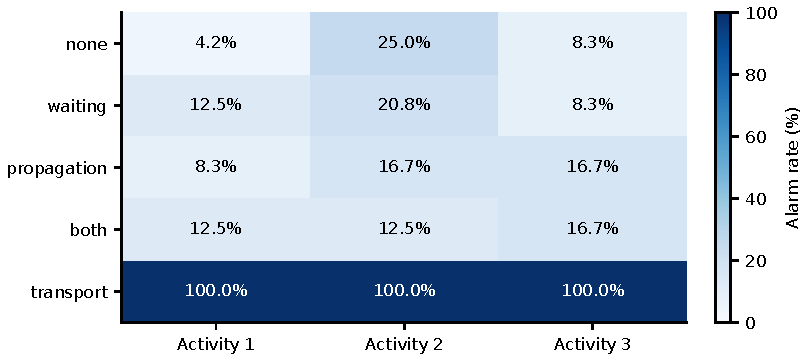
\includegraphics[width=.83\linewidth]{stress_alarms.pdf}
\caption{Full-model post-observation alarm rates on synthetic worlds. The no-shift row is a false-alarm control. Good detection of a large cancellation shock coexists with weak detection of waiting and propagation shifts. Intervals appear in Table~\ref{tab:stress}.}
\label{fig:stress}
\end{figure}
The original evaluator's diagnostic requires both low epistemic variance and RMSE above $0.08$. It never triggers for the waiting and propagation perturbations in this supplement. Table~\ref{tab:stress_magnitude} reports actual truth displacement: the waiting perturbation is small in some templates, so non-detection is not evidence of equal failure severity across shifts. Both diagnostics use realized outcomes and are not advance warnings. Shared agreement among misspecified candidates cannot, by itself, identify a missing rule.

\subsection{RQ2: What improves evidence efficiency, and what is accelerated?}
The original development AUC decreases from \InitialDev\ to \FinalDev, a \DevReduction\% reduction after adaptive selection on the same development set. The frozen test AUC is \TestAUC. This is evidence for the selected predictor on the fixed synthetic evaluation, not a percentage improvement over an external state of the art. The independent-world macro result is a different statistic and must not be substituted for the pooled test score.

Table~\ref{tab:acquisition_original} and the top row of Figure~\ref{fig:curves} show the original comparison. The lower Full curve includes the benefit of evolved calibration, whereas the other selectors start from uniform compatible weights. Under the matched-prior comparison in Table~\ref{tab:acquisition_matched}, the apparent acquisition advantage disappears. Matched-prior Random has macro AUC \MacroRandom, slightly below Full's \MacroFull. The differences are very small, and the near-flat curves indicate that the initially concentrated weights largely determine prediction. These controls prevent attributing calibration gains to the query criterion.
\begin{table}[tbp]
\centering
\caption{Original comparison: calibration and acquisition both vary. Activity AUC $\times10^3$ with 95\% world-bootstrap intervals; 24 worlds, fixed training data, evidence and templates.}
\label{tab:acquisition_original}
\scriptsize
\setlength{\tabcolsep}{3pt}
\begin{tabular}{lrrr}
\toprule
Method & Activity 1 & Activity 2 & Activity 3 \\
\midrule
Random & 17.82 [17.23, 18.39] & 19.03 [18.10, 20.01] & 14.96 [14.46, 15.44] \\
Entropy & 12.94 [12.27, 13.64] & 10.15 [9.21, 11.16] & 8.19 [7.32, 9.14] \\
ParamIG & 12.98 [12.34, 13.68] & 10.80 [10.06, 11.59] & 8.56 [7.50, 9.73] \\
Standard OED & 23.59 [22.32, 24.75] & 27.44 [24.79, 30.05] & 21.58 [19.34, 23.61] \\
Full & 4.19 [3.38, 5.07] & 10.85 [8.78, 12.85] & 6.15 [3.98, 8.65] \\
\bottomrule
\end{tabular}
\end{table}

\begin{table}[tbp]
\centering
\caption{Controlled acquisition comparison: all methods use the evolved prior. Activity AUC $\times10^3$ with 95\% world-bootstrap intervals; 24 worlds, fixed training data, evidence and templates.}
\label{tab:acquisition_matched}
\scriptsize
\setlength{\tabcolsep}{3pt}
\begin{tabular}{lrrr}
\toprule
Method & Activity 1 & Activity 2 & Activity 3 \\
\midrule
Matched-prior Random & 4.19 [3.38, 5.07] & 10.84 [8.77, 12.84] & 6.15 [3.98, 8.65] \\
Matched-prior Entropy & 4.19 [3.38, 5.07] & 10.85 [8.78, 12.85] & 6.15 [3.98, 8.65] \\
Matched-prior ParamIG & 4.19 [3.38, 5.07] & 10.85 [8.78, 12.85] & 6.15 [3.98, 8.65] \\
Matched-prior Standard OED & 4.19 [3.38, 5.07] & 10.85 [8.78, 12.85] & 6.15 [3.98, 8.65] \\
Full & 4.19 [3.38, 5.07] & 10.85 [8.78, 12.85] & 6.15 [3.98, 8.65] \\
\bottomrule
\end{tabular}
\end{table}

\begin{figure}[tbp]
\centering
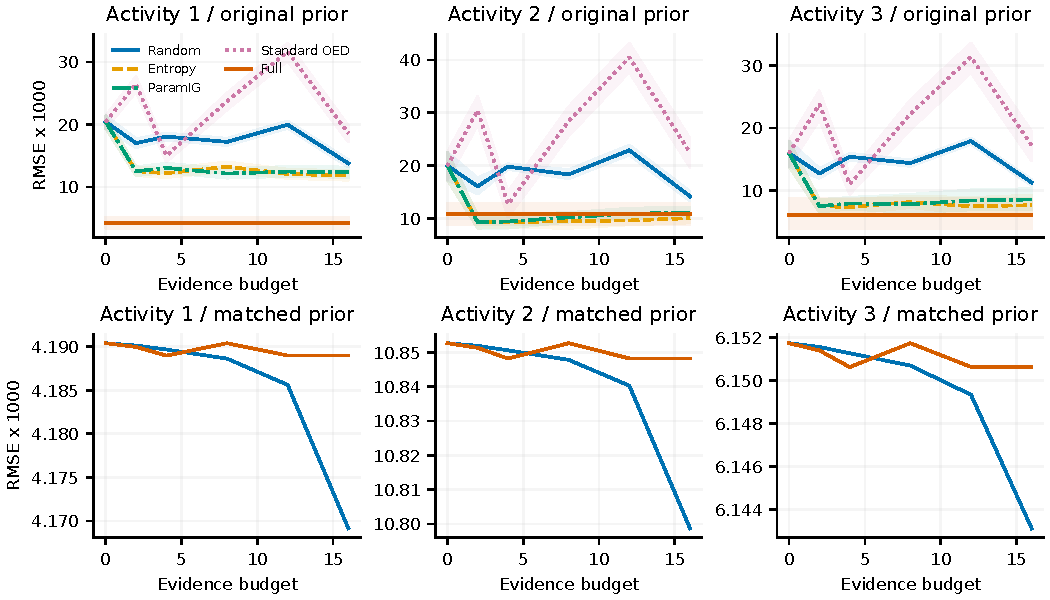
\includegraphics[width=\linewidth]{budget_curves.pdf}
\caption{Synthetic budget--trajectory error curves, reported separately by activity. Top: original calibration policies with conditional 95\% world-bootstrap shading. Bottom: all selectors share the evolved prior; curves nearly coincide. Bottom-row axes retain absolute values but use different scales, so their tiny variations should not be compared visually with top-row effect sizes.}
\label{fig:curves}
\end{figure}

\paragraph{Scoring microbenchmark.}
We compare covariance scoring with explicit enumeration of both binary outcomes, using identical candidates, cached predictions, probabilities, and costs. Ten GPU-synchronized timing pairs alternate execution order. Table~\ref{tab:timing} reports median per-pair speedups of \FrozenSpeed$\times$ under frozen weights and \UniformSpeed$\times$ under uniform compatible weights, with maximum score residuals. Figure~\ref{fig:evolution} displays the raw timings. The reference is the supplied loop-based enumeration implementation; a fully vectorized enumerator can share much of the same work. Accordingly, these measurements establish a local implementation advantage, not a universal speedup over optimized OED or an asymptotic improvement.
\begin{table}[tbp]
\centering
\caption{Ten synchronized, alternating-order GPU timing pairs. Median ratios are computed per pair; they need not equal the ratio of marginal medians.}
\label{tab:timing}
\scriptsize
\setlength{\tabcolsep}{3pt}
\begin{tabular}{lrrrr}
\toprule
Prior & Cov. (ms) & Enum. (ms) & Median ratio & Max. difference \\
\midrule
frozen & 0.773 & 178.17 & 217.95 & 9.08e-16 \\
uniform compatible & 0.747 & 191.85 & 275.16 & 1.38e-10 \\
\bottomrule
\end{tabular}
\end{table}

The canonical full frozen evaluation takes \TestRuntime\ seconds and reports \TestVRAM\ MB of peak allocated PyTorch GPU memory on an RTX 4060 Laptop GPU. These figures concern cached evaluation, excluding offline cache generation and graphics-driver memory. The development trials range from roughly four to nine seconds. Small cached evaluations are feasible on 8 GB VRAM, but this does not demonstrate equivalent scaling for larger populations or richer mechanism banks.

\subsection{RQ3: Which changes survive controlled ablation?}
Table~\ref{tab:ablations} compares the full model with four requested removals and a matched point estimate. Removing the combination target or batch conditioning leaves the aggregate results unchanged. This is consistent with near-single-mechanism weights: altering which evidence is chosen has little effect if the likelihood cannot move substantial mass. Removing sharing worsens results, but its bank uses independent per-event parameter permutations and changes the prior and hypothesis space. The comparison is informative about that implementation, not a pure causal estimate of the benefit of sharing.
\begin{table}[tbp]
\centering
\caption{Frozen-method ablations. Asterisks identify changes that also alter the prior or point-selection objective. Activity AUC $\times10^3$ with 95\% world-bootstrap intervals; 24 worlds, fixed training data, evidence and templates.}
\label{tab:ablations}
\scriptsize
\setlength{\tabcolsep}{3pt}
\begin{tabular}{lrrr}
\toprule
Method & Activity 1 & Activity 2 & Activity 3 \\
\midrule
Full & 4.19 [3.38, 5.07] & 10.85 [8.78, 12.85] & 6.15 [3.98, 8.65] \\
Without sharing* & 47.19 [45.23, 49.01] & 21.17 [18.72, 23.61] & 51.11 [48.60, 53.35] \\
Without combination target & 4.19 [3.38, 5.07] & 10.85 [8.78, 12.85] & 6.15 [3.98, 8.65] \\
Original single point* & 5.42 [4.71, 6.08] & 7.54 [5.92, 9.35] & 7.37 [5.78, 8.95] \\
Matched MAP & 4.19 [3.38, 5.07] & 10.85 [8.78, 12.85] & 6.15 [3.99, 8.65] \\
Without batch conditioning & 4.19 [3.38, 5.07] & 10.85 [8.78, 12.85] & 6.15 [3.98, 8.65] \\
\bottomrule
\end{tabular}
\end{table}


The development history explains the concentration. Rounds 1--7 introduce trajectory weighting and progressively narrow its kernel. Round 30 replaces average historical error with worst-event error. Round 38 narrows the kernel again, but the accepted improvement is only around $10^{-7}$ and should not be presented as a performance leap. Round 58 introduces the noise normalization in Eq.~\eqref{eq:distance}; it produces the largest later improvement. These sequential decisions are not independent ablations, since each accepted change becomes the next parent. All 60 scores and decisions appear in Appendix~\ref{app:trials}.

The aggregate objective also trades off against process prediction: development Brier worsens from \DevBrierStart\ to \DevBrierEnd, and frozen-test Brier is \TestBrier. Frozen-test pointwise coverage is \TestCoverage\% with mean width \TestWidth. High marginal coverage does not establish identified mechanisms or calibrated out-of-model uncertainty. The independent-world uncertainty table (Table~\ref{tab:uncertainty}) separates epistemic and aleatoric contributions; the former is tiny relative to the latter under the selected weights.
\begin{figure}[tbp]
\centering
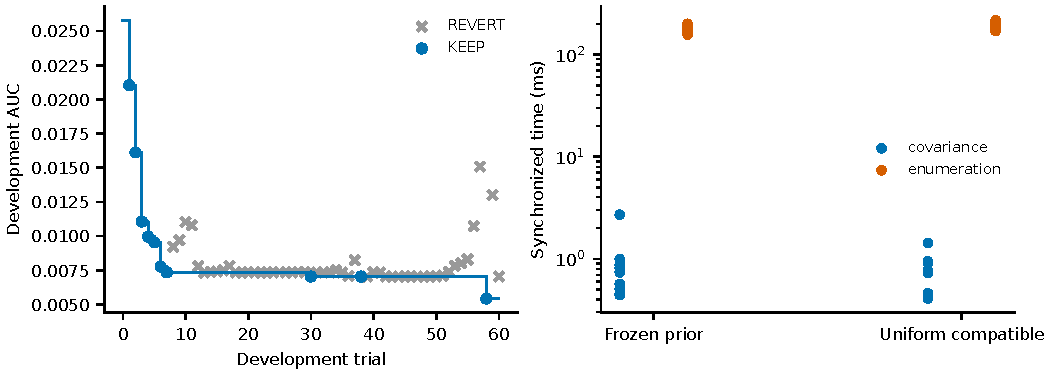
\includegraphics[width=\linewidth]{evolution_timing.pdf}
\caption{Left: all 60 development candidates and the retained-score trajectory. Reverted trials remain visible. Right: all ten timing pairs for each prior; the logarithmic axis distinguishes covariance and explicit enumeration costs without treating timing repetitions as independent activity replicates.}
\label{fig:evolution}
\end{figure}
